% THIS IS AN EXAMPLE DOCUMENT FOR VLDB 2012
% based on ACM SIGPROC-SP.TEX VERSION 2.7
% Modified by  Gerald Weber <gerald@cs.auckland.ac.nz>
% Removed the requirement to include *bbl file in here. (AhmetSacan, Sep2012)
% Fixed the equation on page 3 to prevent line overflow. (AhmetSacan, Sep2012)

\documentclass{vldb}
\usepackage{graphicx}
\usepackage{balance}  % for  \balance command ON LAST PAGE  (only there!)
\usepackage{cleveref}
\usepackage{times}

\newcommand\system{\textsc{SourceSight}}
\newtheorem{definition}{Definition}


\begin{document}

% ****************** TITLE ****************************************

\title{{\LARGE \system}: Enabling Effective Source Selection}

\numberofauthors{3} 

\author{
% 1st. author
\alignauthor
Theodoros Rekatsinas\\
       \affaddr{University of Maryland}\\
       \email{thodrek@cs.umd.edu}
% 2nd. author
\alignauthor
Amol Deshpande\\
       \affaddr{University of Maryland}\\
       \email{amol@cs.umd.edu}
% 3rd. author
\alignauthor 
Xin Luna Dong\\
       \affaddr{Google Inc.}\\
       \email{lunadong@google.com}
\and  % use '\and' if you need 'another row' of author names
% 4th. author
\alignauthor 
Lise Getoor\\
       \affaddr{UC Santa Cruz}\\
       \email{getoor@soe.ucsc.edu}
% 5th. author
\alignauthor Divesh Srivastava\\
       \affaddr{AT\& T Labs-Research}\\
       \email{divesh@research.att.com}
}

\maketitle

\begin{abstract}
Lately there has been a rapid increase in the number of data sources and public access data services, such as cloud-based data markets and data portals, that facilitate the collection, publishing and trading of data. Data sources typically exhibit large heterogeneity in the type and quality of data they provide. Unfortunately, when the number of data sources is large, humans have a limited capability of reasoning about the actual usefulness of sources and the trade-offs between the benefits and costs of acquiring and integrating sources. In this demonstration we present \system, a framework that facilitates the exploration and selection of sources for integration. \system~is based on the intuition that different sets of data sources are optimal to integrate for different integration tasks. The main focus of \system~is on allowing users to discover and explore valuable sets of sources for diverse integration tasks over larger numbers of diverse data sources.
\end{abstract}


\section{Introduction}
Data integration and data cleaning remain among the most cost-intensive tasks in data management, either due to the increased computation and human-labor costs involved in the process~\cite{kruse2015estimating} or the monetary cost involved in acquiring data from different sources~\cite{balazinska:vldb11}. Given the high number of available data sources and the aforementioned costs, it is challenging for a user to identify the sources that are truly beneficial to her application. This gives rise to the natural question of how can one discover {\em the most beneficial sources} for integration, i.e., sources that maximize the user's benefit at the minimum cost. 

Several approaches have been proposed to help users reason about the value of integrating multiple data sources. The proposed approaches can be divided in two main categories: (i) {\em effort-oriented} techniques that focus on characterizing solely the cost of integration, and (ii) data-oriented techniques that reason about the benefit of integration. Techniques from the first category estimate the cost of integration via reasoning about the effort required to perform schema-matching, data-cleaning and data-transformations when integrating multiple sources~\cite{kruse2015estimating, smith:2009}. The main limitation of th Here, the sources are {\em fixed}, assuming that the user has already specified the sources that are relevant to her query and given the estimated integration cost 

describe \system and its unique contributions, i.e., functionalities for the users.

organization of the demo


\section{Discovering Valuable Sources}
We consider a scenario where users interact with a system that stores and manages data sources under a single repository and want to identify sources relevant to a desired integration task. Examples of such repositories may correspond to data marketplaces~\cite{balazinska:vldb11}, data portals, such as Datasift\footnote{http://datasift.com/}, or online platforms for organizing, managing and sharing datasets~\cite{datahub}. 

Sources can exhibit large heterogeneity with respect to the data they provide. We assume that each entry in a source is associated with a set of {\em context literals} and all context literals come from a {\em literal dictionary} $V$. This dictionary $V$ may follow a structured form, e.g., be a knowledge-base, describing how different literals are related to each other. For example, if the source entries correspond to structured entries these literals may correspond to the values for a subset of attributes of each entry (e.g., the location value and business type value for business listings). If the source entry corresponds to unstructured free-text data, these literals may correspond to {\em real-world entities} or {\em concepts} from a knowledge-base. The aforementioned assumptions allow one to reason about the domain covered by each source by analyzing the union of context-literal sets associated with the entries of the source. 

We also consider that a user integration task $I = (I_d, I_c)$ is fully specified by a description that corresponds to a context-literal set $I_d$ defining the {\em domain} of the task and potentially a set of integration cost or effort constraints $I_c$. Discovering the most valuable sources for task $I$ requires performing the following operations: (i) identifying the relevant sources for task $I$, (ii) discovering sets of sources that if integrated together will maximize the {\em benefit} of integration under the constraints $I_c$. 

Relevant sources to task $I$ are all data sources that provide entries whose context-literal set is a subset of $I_d$. Not of all these sources may be beneficial for task $I$ as sources may provide stale or erroneous data~\cite{Dong_vldb:2009, li:2012}, or may provide duplicate data~\cite{bronzi:2013, li:2012} at different prices. In our recent work~\cite{dong:vldb13,rekatsinas:2014, rekatsinas:2015} we showed how
, given a fixed data domain, the benefit of integration can be quantified using rigorous data quality metrics, such as {\em coverage}, {\em accuracy}, {\em timeliness} or {\em bias}, and introduced the paradigm of {\em source selection} to detect the most beneficial sources for integration by reasoning about the benefits and costs of acquiring and integrating data. 

Consider an integration task $I = (I_d, I_c)$ and let $S$ denote the set of all sources relevant to $I$. Assume an oracle $\mathbf{G_q}(\cdot)$ that takes as input a set of sources $\bar{S}$ and a set of context-literals $I_d$ and returns the a vector containing the gain of integrating sources $\bar{S}$ with respect to the different quality metrics $q$. Moreover, let $C(\cdot)$ be an oracle that takes as input a set of sources $\bar{S}$ and returns the total integration cost. The result of source selection corresponds to a sets of sources $S_I$ such that $S_I = \arg\max_{\bar{S} \subseteq S}\mathbf{G_q}(\bar{S},I_d) - C(\bar{S})$.

%\section{Discovering Valuable Sources}
%  We consider a scenario where users interact with a system that stores and manages data sources under a single repository and want to identify sources relevant to a desired integration task. Examples of such repositories may correspond to data marketplaces~\cite{balazinska:vldb11}, data portals, such as Datasift\footnote{http://datasift.com/}, or online platforms for organizing, managing and sharing datasets~\cite{datahub}. In this section we describe the main functionalities that such systems needs to support to allow users to discover sources that are the most beneficial for a desired integration task. 
%
%\subsection{Reasoning about The Content of Sources}
%Sources may exhibit large heterogeneity with respect to the data they provide. To reason about the content of sources we assume that each entry in a source is associated with a set of {\em context literals}. We assume that all context literals come from a {\em literal dictionary} $V$. Moreover, we assume that the dictionary $V$ may follow a structured form, e.g., be a knowledge-base, describing how different literals are related to each other. For example, if the source entries correspond to structured entries these literals may correspond to the values for a subset of attributes of each entry (e.g., the location value and business type value for business listings). If the source entry corresponds to unstructured free-text data, these literals may correspond to {\em real-world entities} or {\em concepts} from a knowledge-base. Following this assumption, a data-source repository can reason about the domain covered by each source by analyzing the union of context-literal sets associated with the entries of the source. 
%
%\subsection{Describing the Integration Task}
%Typically a user would start by proving a description of her desired integration task as well as any requirements (e.g., requirements on the total effort of integration) characterizing the task. We assume that users can describe a desired integration task using a set of context literals that belong in the dictionary $V$. Integration-task requirements can correspond to constraints on the total number of sources used for integration or explicit budget constraints on the cost or total effort of integration.
%
%Given an integration task $I$ described by a  context-literal set $I_c$, the system can {\em recommend}.
%
%
%\subsection{Multi-variate Source Selection}
%Given a finalized integration task $I$ associated with a context-literal set $I_c$ the system automatically finds subsets of sources that, if integrated together, maximize the benefit of integration under the budget requirements of the user. If available, the system identifies multiple solutions that correspond to different trade-offs among different quality metrics.
%
%The discovered solutions are presented to the user together with a concise description of their quality characteristics as well as a description of the data sources included in each of thi think em. 
%
%\subsection{Providing Explanations}
%
%analyze the content of sources, identify the domains that sources cover and materialize quality profiles. 
%
%Different quality metrics available 
%
%Users provide a query that specifies a domain
%
%Oracle provides the quality profiles of sources for the specified domain
%
%Perform source selection

\section{{\Large \system} Design}
In this section, we present \system, a data source management system for effective source selection over large numbers of diverse data sources. In a recent paper~\cite{rekatsinas:2015}, we put forward our vision about the functionalities that data source management systems should support to facilitate effective source selection and the architecture they should follow. 
\system~is a realization of our vision for such a system. Next, we describe \system's architecture, the different functionalities it supports and extensions of the preliminary design implemented in \system.%

\subsection{Architecture overview}
\system-is built as a layer on top of a data source repository, that stores the raw data of data sources. The system consists of three components: a frontend, a source analysis engine and a query engine. The frontend is a ``thin client'' that is used to specify integration tasks and display visualizations that aid users to select the desired sources for integration. The source analysis engine processes the raw data from the available data sources to identify the content of sources, and also evaluates their quality with respect to different quality metrics such as the ones describe in the previous section. Finally, the query engine takes as input user-specified requests and performs the necessary computation to serve those. The architecture of \system~is presented in \Cref{fig:architecture}. 

\begin{figure}[h]
    \centering
    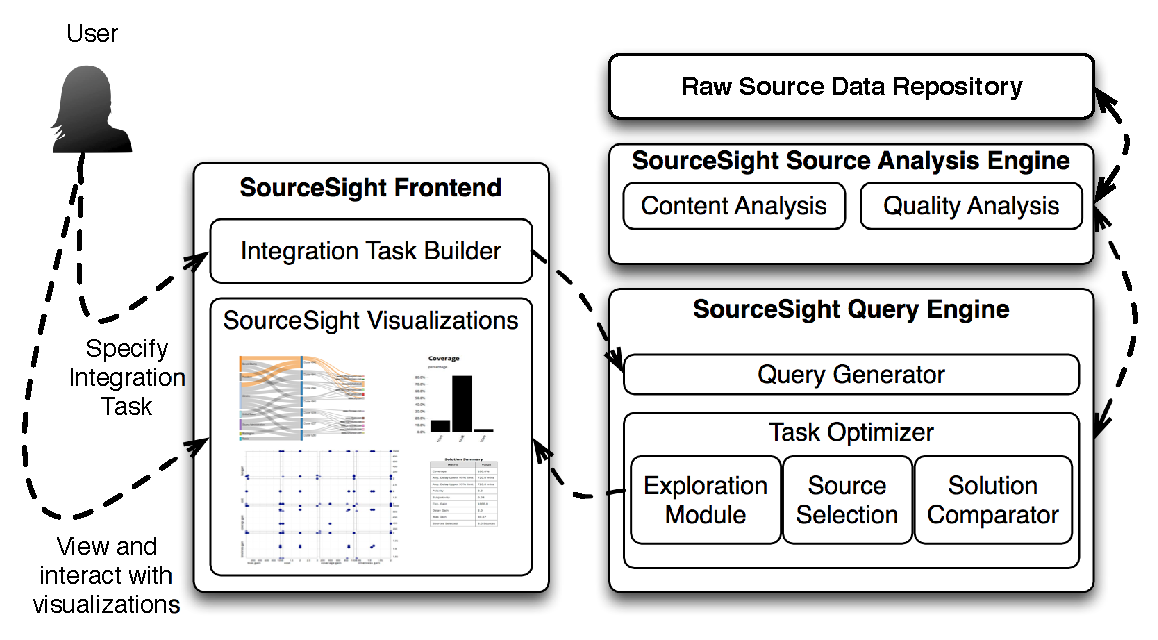
\includegraphics[width=0.5\textwidth]{fig/srcsightOver}
    \caption{\system~architecture.}
    \label{fig:architecture}
\end{figure}

The basic operations of \system can be divided into an {\em offline} phase and an {\em online} phase. During the offline phase, the source analysis module constructs an index describing both the content and the quality of each source with respect to multiple quality metrics. This index is used during the online phase when a user interacts with the system to serve the user requests. We discuss the indexing technique used further in \Cref{sec:reasoning} During the online phase users interact with \system~via its frontend module and user requests are served by the query engine. Users can specify a desired integration task by providing a free-text description of the context literals that describe the task. Once a description is provided users can choose among three main functionalities with respect to the specified integration task. They can either choose to explore which context literals and sources are highly relevant to the specified task, they can choose to perform source selection or they can choose to perform a qualitative comparison between different sets of sources constructed either manually or automatically via source selection. The first functionality allows a user to refine her integration task specification by exploring related contexts. It also allows users to obtain an overview of the quality of individual sources (see \Cref{sec:integtask}). The second functionality returns multiple recommended source selection solutions with respect to a variety of quality metrics (see \Cref{sec:sourcesel}). Finally, \system~allows users to compare and contrast different sets of sources to further understand the benefits of choosing a specific set and understand why the particular set was recommended by source selection (see \Cref{sec:extensions}). We now discuss the different components in detail.

\subsection{Reasoning about The Content of Sources}
\label{sec:reasoning}
Sources may exhibit large heterogeneity with respect to the data they provide. To reason about the content of sources we assume that each entry in a source is associated with a set of {\em context literals}. We assume that all context literals come from a {\em literal dictionary} $V$. Moreover, we assume that the dictionary $V$ may follow a structured form, e.g., be a knowledge-base, describing how different literals are related to each other. For example, if the source entries correspond to structured entries these literals may correspond to the values for a subset of attributes of each entry (e.g., the location value and business type value for business listings). If the source entry corresponds to unstructured free-text data, these literals may correspond to {\em real-world entities} or {\em concepts} from a knowledge-base. Following this assumption, a data-source repository can reason about the domain covered by each source by analyzing the union of context-literal sets associated with the entries of the source. 

\subsection{Specifying and Refining an Integration Task}
\label{sec:integtask}
Typically a user would start by proving a description of her desired integration task as well as any requirements (e.g., requirements on the total effort of integration) characterizing the task. We assume that users can describe a desired integration task using a set of context literals that belong in the dictionary $V$. Integration-task requirements can correspond to constraints on the total number of sources used for integration or explicit budget constraints on the cost or total effort of integration.

Given an integration task $I$ described by a  context-literal set $I_c$, the system can {\em recommend}.


\subsection{Multi-variate Source Selection}
\label{sec:sourcesel}
Given a finalized integration task $I$ associated with a context-literal set $I_c$ the system automatically finds subsets of sources that, if integrated together, maximize the benefit of integration under the budget requirements of the user. If available, the system identifies multiple solutions that correspond to different trade-offs among different quality metrics.

The discovered solutions are presented to the user together with a concise description of their quality characteristics as well as a description of the data sources included in each of thi think em. 

\subsection{Extensions}
\label{sec:extensions}
Next, we discuss two extensions that \system.
\subsubsection{Providing Explanations}

analyze the content of sources, identify the domains that sources cover and materialize quality profiles. 

Different quality metrics available 

Users provide a query that specifies a domain

Oracle provides the quality profiles of sources for the specified domain

Perform source selection

\subsubsection{Comparing and Contrasting Sets of Sources}


\section{Demo Details}

Explore correspondence graph to help users identify the domain of their interest

Get an initial understanding of what's the quality of relevant sources

Perform source selection and identify sets of sources that optimize for different
quality metrics

Compare user constructed solutions with source-selection solutions

Allow users to remove and add sources

\bibliographystyle{abbrv}
\bibliography{srcsight}

\end{document}
